\anothertitle{Results and Discussion}{}

\begin{frame}
  \Frametitle{Viable Solutions}
  \vspace{15pt}
  \begin{itemize}
    \item \bullettext{AWS Lambda (representing \textit{Serverless Functions})}
    \item \bullettext{AWS ECS (representing \textit{Cloud Native})}
          \begin{itemize}
            \item \bullettext{running on EC2 (representing \textit{Virtual Machines})}
            \item \bullettext{running on Fargate (representing \textit{Serverless Containers})}
          \end{itemize}
    \item \bullettext{AWS EKS (representing \textit{Kubernetes})}
          \begin{itemize}
            \item \bullettext{running on EC2 (representing \textit{Virtual Machines})}
            \item \bullettext{running on Fargate (representing \textit{Serverless Containers})}
          \end{itemize}
  \end{itemize}

  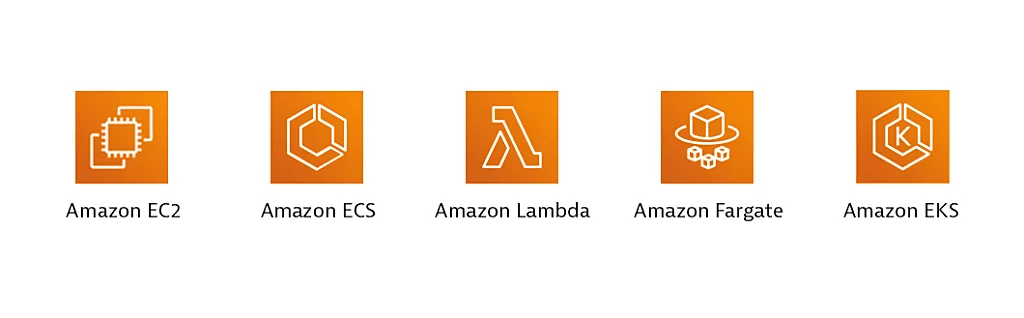
\includegraphics[keepaspectratio,width=\textwidth,height=\textheight]{aws_containerOptions}  
\end{frame}

\begin{frame}
  \Frametitle{Performance and Latency}
  \bullettext{Benchmarks broken up into the following sections:}
  \begin{itemize}
    \item \bullettext{CPU}
    \item \bullettext{Memory}
    \item \bullettext{I/O}
    \item \bullettext{General Workloads}
  \end{itemize}

\end{frame}
\titleimage{CPU - sysbench}{Average time taken to compute primes up to 1000000 --- lower is better}{perf-sysbench}
\titleimage{CPU - 7zip}{Average rating in MIPS --- higher is better}{perf-7zip}
\titleimage{Memory - RAMSpeed}{Average maximum speed achieved --- higher is better}{perf-RAMSpeed}
\titleimage{Memory - MBW}{Average maximum speed achieved --- higher is better}{perf-MBW}
\titleimage{I/O - FSMark}{Average maximum speed achieved --- higher is better}{perf-FSMark}
\titleimage{General Workloads - m-queens}{Average amount of time --- lower is better}{perf-m_queens}
\titleimage{General Workloads - tcb}{Average amount of time to complete (number\_of\_events=30000) --- lower is better}{perf-tcb_network}




\begin{frame}
  \Frametitle{Cost}
  \begin{itemize}
    \item \bullettext{Benchmarked Costing}
    \item \bullettext{Forecasted Costing}
  \end{itemize}
\end{frame}
\titleimage{Cost - Benchmarked}{Average cost of running \emph{tool-container-benchmark} with 30000 events --- lower is better}{cost-workload}

{
  \setbeamertemplate{frametitle}[default][center]
  \addtobeamertemplate{frametitle}{\vskip+1cm}{}
  \begin{frame}
    \frametitle[center]{\LARGE {\textls[90]{\MakeUppercase{Cost - Forecasted}}}}

    \begin{table}[htbp]
      \caption{\emph{Cost}: Projected costing (\$) of running a sample long-lived service per solution for a month and year}
      \small
      \begin{tabularx}{1\textwidth}{X | X | X }
        \space            & \bf{Monthly} & \bf{Annually} \\
        \hline
        \bf{Lambda      } & 120.11       & 1441.32       \\
        \bf{ECS\_Fargate} & 40.99        & 491.88        \\
        \bf{ECS\_EC2    } & 40.623125    & 487.4775      \\
        \bf{EKS\_Fargate} & 113.99       & 1367.88       \\
        \bf{EKS\_EC2    } & 113.623125   & 1363.4775     \\
      \end{tabularx}
    \end{table}

  \end{frame}
}

\begin{frame}
  \Frametitle{Resilience and Reliability}
  \bullettext{Chaos-Engineering:}
  \begin{itemize}
    \item \bullettext{Scaling 1-0-1}
    \item \bullettext{Forcibly killing underlying container}
    \item \bullettext{Rebooting underlying host}
  \end{itemize}
\end{frame}
\titleimage{Resilience and Reliability - Scaling}{Average amount of downtime measured --- lower is better}{rr-scaling}
\titleimage{Resilience and Reliability - Forced Kill}{Average amount of downtime measured --- lower is better}{rr-deleteContainer}
\titleimage{Resilience and Reliability - Host Reboot}{Average amount of downtime measured --- lower is better}{rr-reboot}

\begin{frame}
  \Frametitle{Ease-of-Use}
  \bullettext{Each platform was rated and measured in respect to:}
  \begin{itemize}
    \item \bullettext{Architecture}
    \item \bullettext{Configuration}
    \item \bullettext{Deployment}
    \item \bullettext{Documentation}
  \end{itemize}
\end{frame}
\titleimage{Ease-Of-Use}{Amount of time taken to complete bootstap and convert workload --- lower is better}{eou}